\scanpage{53}
\mspage{\handwritten{21}}
% archive sheet number: 52

$G=\underset{\handwritten{\longleftarrow}}{\lim}G_i$ (EGA IV 8.2 3). \deleted{Le fait que} les morphismes de transition sont fidèle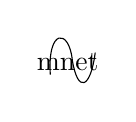
\begin{tikzpicture}[x=1cm,y=1cm,baseline=(n.base)]\node (n) at (0,0) {mnet};\draw (-.22,-.16) .. controls (-.26,.43) and (.02,.43) .. (.06,.02) .. controls (.13,-.4) and (.29,-.34) .. (.35,.12);\end{tikzpicture} plats d'après le lemme suivant :
% A handwritten transposition mark joins the n and e of the line-end continuation.


\uline{Lemme 11.14.- Soient $k$ un corps, $G$ et $H$ deux $k$-groupes affines de type fini, $u:G\handwritten{\longrightarrow}H$ un morphisme de $k$-groupes, et $u^{\unsure{o|0|\circ}}:B\handwritten{\longrightarrow}A$ l'homomorphisme de $k$-algèbres correspondant . Pour que $u$ soit fidèlement plat, il faut et il suffit que $u^o$ soit injectif.}

la condition est évidemment nécessaire (EGA IV 2.2.3 et $\unsure{0|O}_{\mathrm{IV}}$ 6.6.1). Montrons qu'elle est suffisante. Posons $K=\operatorname{Ker}u$. Alors $G/K$ est un $k$-groupe\inserted{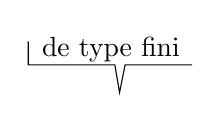
\begin{tikzpicture}[x=1cm,y=1cm,baseline=(n.base)]\node (n) at (0,0) {de type fini};\draw (-1.05,.1)--(-1.05,-.2)--(.05,-.2)--(.11,-.55)--(.18,-.2)--(1.03,-.2);\end{tikzpicture}} (\deleted{Exp.} $\mathrm{VI}_A$ 5.2), et $u$ se factorise en $G\overset{\inserted{p}}{\handwritten{\longrightarrow}}\deleted{p}G/K\overset{v}{\handwritten{\longrightarrow}}H$, où $p$ est fidèlement plat (\deleted{Exp.} $\mathrm{VI}_A$ 3.2) et où $v$ est un monomorphisme de $k$-groupes de type fini, donc une immersion fermée (1.4.2). Puisque $H$ est un schéma affine, et que $v$ est une immersion fermée, $G/K$ est un schéma affine (\unsure{FGA|EGA} I 4.2.3), et, si on note $C$ l'algèbre de $G/K$, l'homomorphisme $v^o:B\handwritten{\longrightarrow}C$ est surjectif (loc. cit.) Or, puisque $u^o$ est injectif, et que $u^o=p^o\mathbin{o}v^o$, $v^o$ est aussi injectif : c'est un isomorphisme, donc $v$ est un isomorphisme, et, puisque $p$ est fidèlement plat, il en est de même de $u$.

\uline{Définitions 11.15}.- Etant donné un corps $k$, un $k$-espace vectoriel $V$, un $k$-groupe $G$ opérant sur $V$, et un vecteur $v\in V$, on dit que $v$ est \uline{semi-invariant} sous $G$ si le sous-espace vectoriel $\handwritten{k.v}$ \deleted{soit}\handwritten{est} stable sous $G$.
\margin{\figure{\handwritten{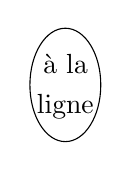
\begin{tikzpicture}[x=0.45cm,y=0.45cm]\draw (0,0) ellipse (1 and 1.6);\node at (0,0.6) {à la};\node at (0,-0.6) {\unsure{ligne}};\end{tikzpicture}}}}
\figure{\handwritten{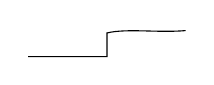
\begin{tikzpicture}[x=0.5cm,y=0.3cm]\draw (0,0) -- (2,0) -- (2,1) .. controls (2.5,1.2) and (3.3,1) .. (4,1.1);\end{tikzpicture}}}
Notons $A$ l'algèbre de $G$, et $\handwritten{\rho}:V\handwritten{\longrightarrow}A\handwritten{\otimes}_k V$ l'application linéaire qui définit l'opération de $G$ sur $V$. Dire que $v$ est semi-invariant sous $G$ revient à dire \deleted{que, pour} qu'il existe $\handwritten{\lambda}\in A$ tel que, pour tout $w\in kv$, $\handwritten{\rho}(w)=\handwritten{\lambda\otimes}w$. Lorsque $v\handwritten{\neq}0$, l'élément $\handwritten{\lambda\in}A$ est bien déterminé par cette relation, on l'appellera \deleted{\uline{invariant}}\inserted{\handwritten{\uline{poids}}} de l'élément semi-invariant $\handwritten{v}$.

\deleted{D'autre part, $v$ s'interprète comme un élément du bidual de $V$, donc comme une section de $\handwritten{\unsure{\mathbb{V}|V}}(V)$; notons $\handwritten{\varphi}:G\handwritten{\times\mathbb{V}}(V)\handwritten{\longrightarrow\mathbb{V}}(V)$ le morphisme définissant l'opération de $G$ sur $\handwritten{\mathbb{V}}$.} Dire que $v$ est semi-invariant \deleted{revient à dire qu'il existe $\unsure{g\in k|\lambda\in k}$} d'invariant $\handwritten{\lambda}$ revient à dire que $\handwritten{\varphi}(g,v)=\handwritten{\unsure{\lambda|\widetilde{\lambda}|\chi}}(g)v$ pour tout $g\in G(k)$, où $\deleted{\handwritten{\unsure{\chi:G\longrightarrow\underline{G}_{m,k}}}}\inserted{\handwritten{\lambda:G\longrightarrow\underline{G}_{m,k}}}$ est le morphisme défini par $\handwritten{\lambda}$. On voit donc que $\handwritten{\lambda}$ \deleted{correspond à}\inserted{\handwritten{est}} un caractère \deleted{\handwritten{\unsure{$\chi$}}} de $G$, appelé \uline{caractère associé} à l'élément semi-invariant $v$. \deleted{Enfin nous appellerons poids de l'élément semi-invariant $v$ le poids du caractère $\handwritten{\chi}$ associé à $v$.}
\margin{\handwritten{!}}
